%%
%% tutorial.tex
%% 
%% Made by Roberto Cavada
%% Login   <cavada@localhost.localdomain>
%% 
%% Started on  Wed Dec 20 14:54:14 2006 Roberto Cavada
%%


\documentclass{article}

\usepackage{epsfig}
\usepackage{graphicx}
\usepackage{xspace}
\usepackage{url}
\usepackage{color}

\newcommand{\kw}[1]{\emph{#1}\xspace}

\newcommand{\appl}[1]{\textsl{#1}\xspace}

\newcommand{\swig}{\appl{Swig}}

\newcommand{\glade}{\appl{Glade}}

\newcommand{\pygtk}{\appl{PyGTK}}
\newcommand{\python}{\appl{Python}}

\newcommand{\mvco}{\kw{MVC--O}}
\newcommand{\mvc}{\kw{MVC} pattern\xspace}
\newcommand{\obs}{\kw{Observer} pattern\xspace}
\newcommand{\gui}{\kw{GUI}}
\newcommand{\pygtkmvc}{\kw{pygtkmvc}}


\newcommand{\file}[1]{\texttt{#1}\xspace}

\definecolor{codecolor}{rgb}{0.1,0,0.4}

\newcommand{\codename}[1]{\texttt{\bfseries \textcolor {codecolor}{#1}}\xspace}

\newcommand{\codesize}{\small } %%\color{codecolor}}
\newcommand{\vc}{\kw{V\&C}}

\begin{document}

\title{A short tutorial for \pygtkmvc\\
Version 1.2.0}

\author{ Roberto Cavada \thanks{ITC-irst, Trento, Italy,
 cavada@irst.itc.it} }

\maketitle

\tableofcontents
\newpage

\section{What is this?}
\pygtkmvc is a practical implementation of \mvc and \obs. The goal of
this tutorial is to provide readers with sufficient awareness about
what \pygtkmvc is and what it can do, in order to allow them to
quickly decide whether it might be useful or not for their needs.

The tutorial is thought to be minimal, meaning that many of provided
features are not mentioned. For any further information the user
should refer to the manual pages.


\section{The example in few words}
The sample application must provide a single window, with a label
showing the value of a numeric counter. The window contains also a
button, which increments the counter by one every time it is pressed.

\begin{figure}[htbp]
\begin{center}
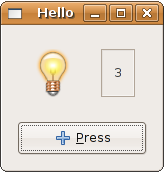
\includegraphics[width=3cm]{eps/appl}
\caption{How the mini-application looks like}
\end{center}
\end{figure}


Since this tutorial must fit into few pages, the example is extremely
simple. Moreover, a more convoluted example would not help to better
understand what \pygtkmvc can be used for.


\section{The framework}
The implementation of this example is split into three distinct
parts. First, the \gui is constructed from a \glade file. Second,
the \gui is constructed \emph{by hand}, by creating and connecting
manually all widgets. Third, adapters are applied to make the code
much more easy.

Hand-made view is mainly presented to make this tutorial more
complete, but the readers should keep in mind that they are going to
adopt the former most of the times, or even more often a mixture of
them, where many parts come from one or more glade files, and some
others are built manually.

The use of glade files is also the reason why the \pygtkmvc framework
is split into three distinct parts. It is a matter of fact that in
practice the Model-View-Controller pattern will almost always collapse
to a two-level framework, where the View and the Controller are
represented by a unique monolithic entity (let's call it \vc),
and the Model is still separated by the rest.

The \pygtkmvc framework provides three well-distinguishable levels, to
allow the pure-glade parts to go into the View side (in a direct and
very natural way), and all the remaining parts that would be put in
the \vc part, to go either in the Controller part, or in the View
part, depending on how much close to the \gui stuff are.

For example, all the widgets signal handlers must go in the Controller
side, whereas the code that sets some attributes of a specific widget
might live either in the Controller or in the View, depending on how
much those attributes are bounded to the application logic.

The more some code depends on the logic of the application, the
farther it lives from the View side. If some code depends only on the
logic without any relation with the \gui stuff, it must live in the
Model.


\section{The implementation glade-based}

\subsection{The model}
The model is represented by class \codename{MyModel}, derived from
class \codename{Model}, that in turn is provided by the framework.

The class \codename{MyModel} contains a field called
\codename{counter} to hold the value of a numeric counter. Since we
are interested in monitoring and show any change of this counter, we
declare it as an \emph{observable property}.


{ \codesize 
\begin{verbatim}   
from gtkmvc.model import Model

class MyModel (Model):
    # observable properties:
    __properties__ = { 'counter' : 0 }

    def __init__(self):
        Model.__init__(self)
        return

    pass # end of class
\end{verbatim}
} 

All that it is required to do, is calling class \codename{Model}'s
constructor from within the derived class' constructor, and defining a
class variable \codename{\_\_properties\_\_} containing the name of the
observable properties, and the associated initial values. The base
class \codename{Model} will do all the boring work automatically.



\subsection{The glade-based view}
\glade while editing the example is depicted in figure
\ref{fig:glade}. The names for the main window, the label and the
button are significant, and signal clicked of the button has been
associated with a function called \codename{on\_button\_clicked}.

\begin{figure}[htbp]
\begin{center}
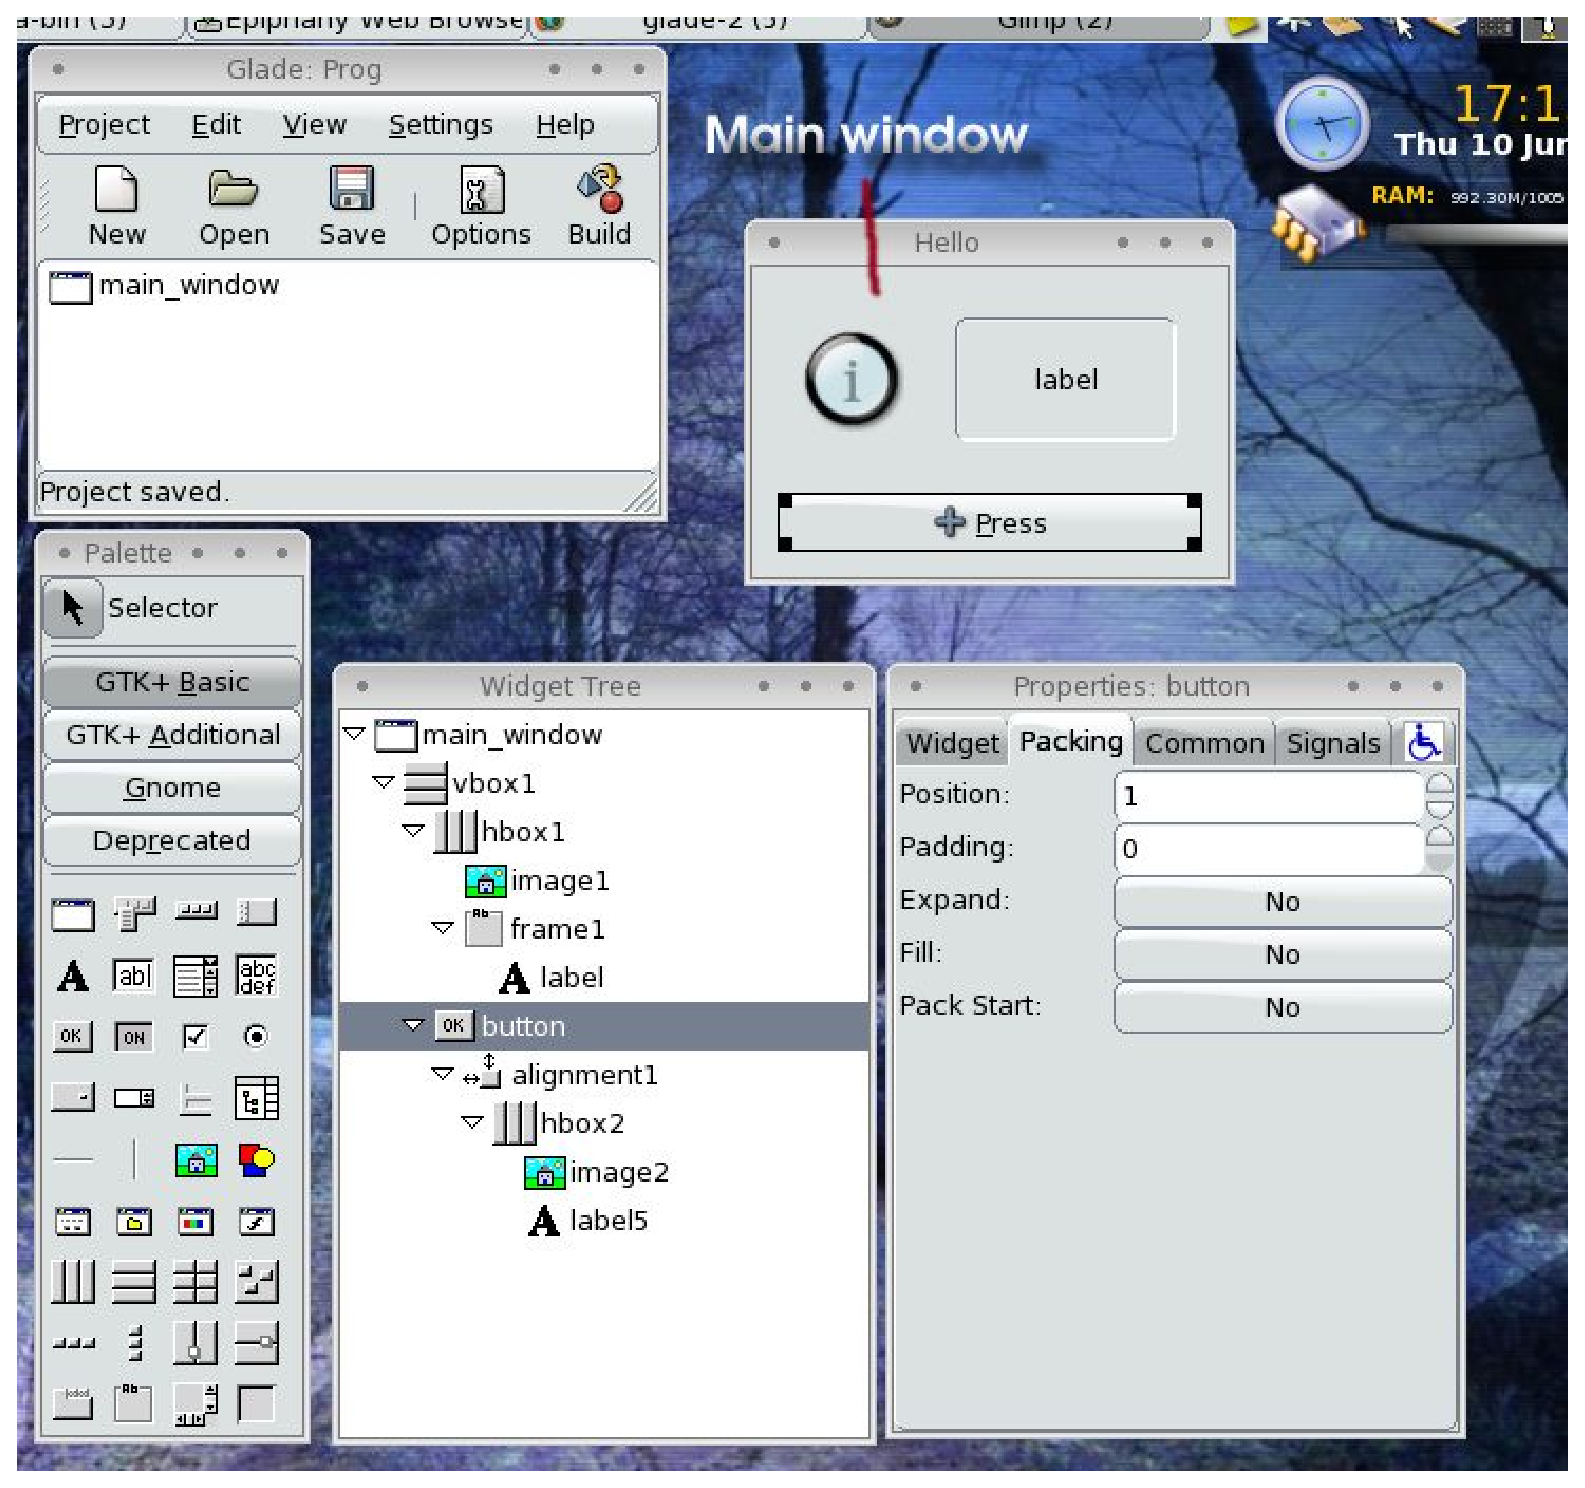
\includegraphics[width=10cm]{eps/glade}
\caption{\label{fig:glade}\glade at work}
\end{center}
\end{figure}


The result is saved in file \file{pygtkmvc-example.glade}.

The view is represented by class \codename{MyView}, that derives from
class \codename{View} provided by \pygtkmvc. The class \codename{View}
can be thought as a container that holds a set of widgets, and may
associate each widget with a string name. When a glade file is used to
build the view, each widget will be associated automatically inside
the view with the corresponding name occurring in the glade file.

Moreover, each \codename{View} instance is connected to a
corresponding \codename{Controller}, and when built from a glade file,
methods inside the \codename{Controller} will be scanned to try to
connect automatically all signals declared in the glade file.

{ \codesize 
\begin{verbatim}   
from gtkmvc.model import Model
  
# This is file model.py
from gtkmvc.view import View

class MyView (View):

    def __init__(self, ctrl):
        View.__init__(self, ctrl, 'pygtkmvc-example.glade')
        return

    pass # end of class
\end{verbatim}
}

Class \codename{MyView} calls simply \codename{View}'s class
constructor from within its constructor, by passing the
\codename{Controller} instance which it belongs to, and the glade file
name. All the hard work is carried out by class \codename{View}.


\subsection{The controller}
The controller - so to speak - is the most complicated part of this
example. It is the only part of the \mvc which knows the model and the
view instances which it is linked to. These are accessible via members
\codename{self.model} and \codename{self.view} respectively.
  
{ \codesize 
\begin{verbatim}   
# This is file ctrl_glade.py
from gtkmvc import Controller
import gtk

class MyController (Controller):
    def __init__(self, model):
        Controller.__init__(self, model)

        # The controller is an observer for properties contained in
        # the model:
        return

    def register_view(self, view):
        """This method is called by the view, that calls it when it is
        ready to register itself. Here we connect the 'pressed' signal
        of the button with a controller's method. Signal 'destroy'
        for the main window is handled as well."""

        Controller.register_view(self, view)

        # connects the signals:
        self.view['main_window'].connect('destroy', gtk.main_quit)
        
        # initializes the text of label:
        self.view['label'].set_text("%d" % self.model.counter)
        return
       
    # signals:
    def on_button_clicked(self, button):
        self.model.counter += 1  # changes the model
        return

    # observable properties:
    def property_counter_value_change(self, model, old, new):
        self.view['label'].set_text("%d" % new)
        print "Property 'counter' changed value from %d to %d" % (old, new)
        return
    
    pass # end of class
\end{verbatim}
} 

In the class constructor, at first base class constructor is called,
passing the \codename{Model} instance this \codename{Controller}
instance belongs to. From that moment on, class member self.model will
be accessible.

\codename{Controller}'s base class \codename{Observer} calls method
\codename{Model.register\_observer} in order to make the controller
an observer for the observable property \codename{counter} in the
model. After this, every change applied to \codename{MyModel} class'
member \codename{counter} will make method
\codename{property\_counter\_value\_change} of class \\
\codename{MyController} be called automatically.

Method \codename{register\_view} is called when a class
\codename{View} instance requires to be registered to the controller
it belongs to.  This method is mainly used to connect signals and
initialize the \gui side that depends on the application logic. In
the example, signal \codename{"destroy"} of the main window is
connected to \codename{gtk.main\_quit} to close the application when
the user closes the window. Notice here the use of member
\codename{self.view} and how a class \codename{View} can be used as
a map to retrieve widgets from their names.

Also, the text label is initialized to the initial value of the
counter.

Method \codename{on\_button\_clicked} is called as a callback every
time the user clicks the button. The corresponding signal is
automatically connected to this method when class \codename{MyView}
registers itself within the controller.

Finally, method \codename{property\_counter\_value\_change} is
called when the property counter in class \codename{MyModel}
changes. The model containing the property, the old value and the
new value are passed to this method. Notice that the model is passed
since the controller might be an observer for more than one model,
even different from the model it is directly connected to in the
\mvc chain.


\subsection{The main code}
Main code is pretty trivial:
  
{ \codesize 
\begin{verbatim}   
# This is file main_glade.py
import gtk
from model import MyModel
from ctrl_glade import MyController
from view_glade import MyView

m = MyModel()
c = MyController(m)
v = MyView(c)

gtk.main()
\end{verbatim}
} 

A triple MVC is created, and main loop is started. 


\section{The implementation without glade}

\subsection{The model}
The model does not depend on the controller+view sides, so it is
exactly the same as for the implementation glade-based.

\subsection{The view}
Using manually constructed views is slightly less intuitive that using
glade-based views, since the architecture of the view-side \pygtkmvc
is mainly designed to be used with glade files.

{ \codesize 
\begin{verbatim}   
# This is file view_no_glade.py
from gtkmvc.view import View
import gtk

class MyViewNoGlade (View):

    def __init__(self, ctrl):

        # The view here is not constructed from a glade file.
        # Registration is delayed, and widgets are added manually,
        # later.
        View.__init__(self, ctrl, register=False)
    
        # The set of widgets:
        w = gtk.Window()
        h = gtk.VBox()
        l = gtk.Label()
        b = gtk.Button("Press")
        h.pack_start(l)
        h.pack_end(b)
        w.add(h)
        w.show_all()

        # We add all widgets we are interested in retrieving later in
        # the view, by giving them a name. Suppose you need access
        # only to the main window, label and button.  Widgets are
        # added like in a map:
        self['main_window'] = w
        self['label'] = l
        self['button'] = b
        
        # View's registration was delayed, now we can proceed.
        # This will allow the controller to set up all signals
        # connections, and other operations:
        ctrl.register_view(self)

        return

    pass # end of class
\end{verbatim}
} 

The entire work is carried out by the class constructor. At the
beginning base class \codename{View} is called like in glade-based
view class, but now parameter \codename{register} is set to
\codename{False}, to delay the registration of the view within the
controller. This to allow manual construction of the widgets set, that
later during registration the controller will be able to access.

Following lines are used to build the widgets set, and to associate a
few of them with string names (only those that will have to accessed
later).

Finally, last line calls method \codename{register\_view} of the
controller, in order to at last allow the controller to know about
this view.

Notice that here \glade file has not been used at all. Nevertheless, a
mixed solution where \glade file(s) and manually constructed widgets
sets is fully supported.

\subsection{The controller}
The controller is the same that has been used for the glade-based
version, a part from a further signal connection that is performed to
connect the button ``\codename{clicked}'' event to class method
\codename{self.on\_button\_clicked}. For this reason, class
\codename{MyControllerNoGLade} is derived from class
\codename{MyController} to reduce typing.
 
{ \codesize 
\begin{verbatim}   
# This is file ctrl_no_glade.py
from ctrl_glade import MyController

class MyControllerNoGlade (MyController):
    def __init__(self, model):
        MyController.__init__(self, model)
        return

    def register_view(self, view):
        MyController.register_view(self, view)

        # connects the signals:
        self.view['button'].connect('clicked', self.on_button_clicked)
        return    
    
    pass # end of class
\end{verbatim}
} 


\subsection{The main code}
Like previous version, main code for manually built view is very
short:

{ \codesize 
\begin{verbatim}     
# This is file main_no_glade.py
import gtk
from model import MyModel
from ctrl_no_glade import MyControllerNoGlade
from view_no_glade import MyViewNoGlade

m = MyModel()
c = MyControllerNoGlade(m)
v = MyViewNoGlade(c)
gtk.main()
\end{verbatim}
} 

\section{Multiple views, one model}
This example shows the powerful of the \obs.

Here both the glade-based and manually built versions are being run at
the same time, with a single instance of class \codename{MyModel}
shared between those two versions. The execution of this example
results in two windows being displayed; by clicking the button of one
of them, the counter is incremented, and the labels in both of them
are updated.

{ \codesize 
\begin{verbatim}       
# This is file main_mixed.py
import gtk
from model import MyModel
from ctrl_no_glade import MyControllerNoGlade
from ctrl_glade import MyController
from view_no_glade import MyViewNoGlade
from view_glade import MyView

m = MyModel()
c1 = MyControllerNoGlade(m)
c2 = MyController(m)
v1 = MyViewNoGlade(c1)
v2 =  MyView(c2)
gtk.main()
\end{verbatim}
}


\section{Using Adapters}
Since version 1.2 adapters largely contribute to make the code
simpler and so to reduce development costs and efforts.

\smallskip
Adapters \emph{adapt} some part of the model to some part of the
view. In a simple version, one adapter makes one property (possibly
observable) into the model communicate autonomously with a single
widget into the view, and viceversa. Readers can find all
information about adapters in the user manual.

\bigskip
We want to have an adapter to handle coordination between property
\codename{counter} and the label. Model and View remain
unchanged. It is the Controller that can be simplified as follows:

{ \codesize 
\begin{verbatim}   
# This is file ctrl_glade_adap.py
from gtkmvc import Controller
import gtk

class MyControllerAdap (Controller):
    def register_view(self, view):
        Controller.register_view(self, view)
        # connects the signals:
        self.view['main_window'].connect('destroy', gtk.main_quit)
        return

    def register_adapters(self):
        self.adapt("counter", "label")
        return
       
    # signals:
    def on_button_clicked(self, button):
        self.model.counter += 1  # changes the model
        return    
    pass # end of class
\end{verbatim}
} 

Controller method \codename{register\_adapters} is called by the
framework when adapters can be instantiated. The controller is no
longer interested in observing property \codename{Counter} and to
initialize the value shown in the label, as these activities are now
transparently carried out by the adapter.

Notice that if editable widget like a text entry were used instead
of a label, the adapter would also have taken care about changes of
the text entry reporting them to the property. 

\bigskip
Now suppose you want to apply some customization to the way the
label shows the property's value. Method
\codename{register\_adapters} might be:

{ \codesize 
\begin{verbatim}   
    from gtkmvc import adapters
    def register_adapters(self):
        a = adapters.Adapter(self.model, "counter")
        a.connect_widget(self.view['label'], 
             setter=lambda w,v: 
               w.set_markup("<big>Counter=<b>%02d</b></big>" % v))
        self.adapt(a)
        return
\end{verbatim}
} 

\begin{figure}[htbp]
\begin{center}
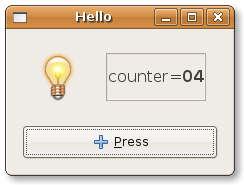
\includegraphics[width=4cm]{eps/adap}
\caption{\label{fig:adap}Adapter at work}
\end{center}
\end{figure}

Here an adapter is created explicitly, and parameter
\codename{setter} is used to custom the functional block that is in
charge of writing to the widget.

There are several types of adapters that can be used, depending on
the property kind and the widget type they adapt. Adapter offer a
very straight and simple default support, but they can be largely
customized when needs get more advanced. See the user manual for
further information.


\section{Generating a standard project from scratch}

Since version 1.2.0 a little application called \kw{gtkmvc-progen}
is available to help setting up from scratch a new application based
on \pygtkmvc. \kw{gtkmvc-progen} is available both as a command-line
program and as a GUI application. 

\begin{figure}[htbp]
\begin{center}
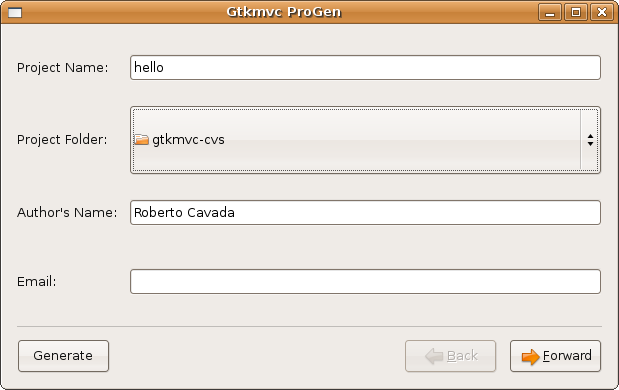
\includegraphics[width=8cm]{eps/progen}
\caption{\label{fig:progen}\kw{gtkmvc-progen} GUI at work}
\end{center}
\end{figure}

By the way, the source code of \kw{gtkmvc-progen} is simple and can
be exploted to learn more about gtkmvc-based applications. A model
carries out all the work, and a controller/view pair provides the
GUI if needed.

\kw{gtkmvc-progen} can be executed either locally from the script
directory, or can be executed as any other program if \pygtkmvc has
been officially installed on the hosting system.

From the local script directory:
\begin{verbatim}
$> python gtkmvc-progen name=hello author="Roberto Cavada" gui=no
\end{verbatim}

If \pygtkmvc was installed:
\begin{verbatim}
$> gtkmvc-progen name=hello author="Roberto Cavada" gui=no
\end{verbatim}

``name=hello'' is an example of setting of a property that customizes the
way \kw{gtkmvc-progen} works. See the user manual for a full list. 

A new directory called \file{hello} will be created in the current
directory (as property \kw{destdir} is ``.'' by default. 

Let us run now the resulting application skeleton.

\begin{verbatim}
$> cd hello
$> ls
hello.py  resources  src

$> python hello.py
\end{verbatim}


\begin{figure}[htbp]
\begin{center}
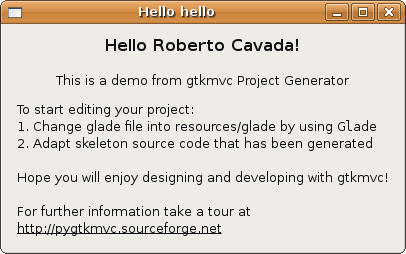
\includegraphics[width=6cm]{eps/hello}
\caption{\label{fig:hello}The skeletal hello application}
\end{center}
\end{figure}


\section{Conclusions}
The author does hope that this tutorial will be useful to help those
who are unsettled about whether \pygtkmvc can fit their needs or not.

Even if very simple, from this tutorial should result clear to the
reader that both the MVC and Observer patterns can strongly improve
the quality of middle and big size \gui applications, especially if
combined with the use of glade-based views.

\pygtkmvc has been extensively used to produce a few large \gui
applications based on \python and \pygtk. In this scenario, many
design choices that led to \pygtkmvc had been determined from
practical needs, and this made easiness and transparency the most
appreciated quality of the framework.

For any further information, and a detailed list of supported
features, please refer to the user manual. 



\end{document}
